\section{Fuentes de datos}

La unidad básica de análisis empleada en este estudio es la parcela, entendida como una superficie geográfica delimitada correspondiente a terrenos forestales definidos en el Inventario Forestal Nacional. Cada parcela está georreferenciada mediante coordenadas precisas, lo cual permite su identificación inequívoca en el espacio. Vemos las parcelas estudiadas en la Figura \ref{fig:parcelas}.

\begin{figure}[H]
    \centering
    \includegraphics[width=0.8\textwidth]{figuras/mapa_parcelas.png}
    \caption{\small Imagen del mapa peninsular con las parcelas contempladas representadas. Las islas Canarias no aparecen en la imagen pero sí que se contemplan en la base de datos.}
    \label{fig:parcelas}
\end{figure}

\subsection{Datos meteorológicos}
Los datos meteorológicos consisten en temperaturas (tanto de la superficie como del suelo) y cantidad de precipitaciones.

\subsubsection*{Temperaturas}

Los datos de temperaturas empleados provienen del dataset \textit{ERA5-Land Daily Aggregated - ECMWF Climate Reanalysis}, procedentes del \textit{Climate Data Store} de Copernicus \cite{copernicus_api} y accedidos a través de Google Earth Engine \cite{copernicus_era5_land_daily}. Este conjunto de datos cubre toda la superficie terrestre de forma continua desde el $1950$ hasta el presente, actualizandose con un margen de $2$ a $3$ meses y recopila información de diversas fuentes, como datos en tierra, satélites o globos meteorológicos. Proporciona una serie temporal de datos en una cuadrícula de latitud-longitud, con una cobertura horizontal global y vertical a varios niveles de profundidad, desde el suelo hasta aproximadamente $200$ cm bajo la superficie. La resolución horizontal es de $0.1^\circ \times 0.1^\circ$, lo que equivale a alrededor de $10$ km.

\medskip

Los datos se pueden descargar a través de la API del \textit{Climate Data Store} (CDSAPI) \cite{copernicus_api} o a través de Google Earth Engine \cite{copernicus_era5_land_daily}. Las variables extraídas se pueden están recogidas en la tabla \ref{tab:era5_land}.



\subsubsection*{Precipitaciones}

Los datos de precipitaciones empleados provienen del dataset \textit{ERA5-Land Daily Aggregated - ECMWF Climate Reanalysis}, procedentes del \textit{Climate Data Store} de Copernicus \cite{copernicus_api} y accedidos a través de Google Earth Engine \cite{copernicus_era5_land_daily}. Este conjunto de datos cubre toda la superficie terrestre de forma continua desde el $1950$ hasta el presente, actualizandose con un margen de $2$ a $3$ meses y recopila información de diversas fuentes, como datos en tierra, satélites o globos meteorológicos. Proporciona una serie temporal de datos en una cuadrícula de latitud-longitud, con una cobertura horizontal global y vertical a varios niveles de profundidad, desde el suelo hasta aproximadamente $200$ cm bajo la superficie. La resolución horizontal es de $0.1^\circ \times 0.1^\circ$, lo que equivale a alrededor de $10$ km..

Los datos se pueden descargar a través de la API del \textit{Climate Data Store} (CDSAPI) \cite{copernicus_api}. Las columnas empleadas se puede ver en la Tabla \ref{tab:era5_land}.


    \begin{table}[H]
\centering
\renewcommand{\arraystretch}{1.5} % Aumenta la separación entre las filas
\resizebox{\columnwidth}{!}{%
\begin{tabular}{|m{5cm}|m{2cm}|m{1cm}|m{8cm}|} % Columnas con ancho fijo y centrado vertical
\cline{1-4}
\multicolumn{4}{|c|}{\cellcolor[HTML]{D9EAD3}{\color[HTML]{000000} ERA5-Land Daily Aggregated - ECMWF Climate Reanalysis}} \\
\cline{1-4}
\multicolumn{1}{|c|}{\cellcolor[HTML]{D9EAD3}{\color[HTML]{000000} Nombre de la variable}} &
  \multicolumn{1}{c|}{\cellcolor[HTML]{D9EAD3}{\color[HTML]{000000} Unidades}} &
  \multicolumn{1}{c|}{\cellcolor[HTML]{D9EAD3}{\color[HTML]{000000} Tipo de datos}} &
  \multicolumn{1}{c|}{\cellcolor[HTML]{D9EAD3}{\color[HTML]{000000} Descripción}} \\
\cline{1-4}
\centering {\color[HTML]{202124} temperature\_2m} &
  \centering {\color[HTML]{202124} K} &
  \centering float &
  {\color[HTML]{202124} Temperatura del aire a 2 m sobre la superficie de la tierra, el mar o las aguas interiores. La temperatura a 2 m se calcula interpolando entre el nivel más bajo del modelo y la superficie de la Tierra, teniendo en cuenta las condiciones atmosféricas.} \\ \cline{1-4}
\centering {\color[HTML]{202124} skin\_temperature} &
  \centering {\color[HTML]{202124} K} &
  \centering float &
  {\color[HTML]{202124} Temperatura de la superficie de la Tierra. La temperatura cutánea es la temperatura teórica necesaria para satisfacer el equilibrio de energía superficial. Representa la temperatura de la capa superficial superior, que no tiene capacidad calorífica y, por lo tanto, puede responder instantáneamente a los cambios en los flujos de superficie. La temperatura cutánea se calcula de manera diferente en tierra y mar.} \\ \cline{1-4}
\centering {\color[HTML]{202124} soil\_temperature\_level\_1} &
  \centering {\color[HTML]{202124} K} &
  \centering float &
  {\color[HTML]{202124} Temperatura del suelo en la capa 1 (0 a 7 cm) del Sistema Integrado de Previsión del ECMWF.} \\ \cline{1-4}
\centering {\color[HTML]{202124} soil\_temperature\_level\_2} &
  \centering {\color[HTML]{202124} K} &
  \centering float &
  {\color[HTML]{202124} Temperatura del suelo en la capa 2 (7-28 cm) del Sistema Integrado de Previsión del ECMWF.} \\ \cline{1-4}
\centering {\color[HTML]{202124} soil\_temperature\_level\_3} &
  \centering {\color[HTML]{202124} K} &
  \centering float &
  {\color[HTML]{202124} Temperatura del suelo en la capa 3 (28 a 100 cm) del Sistema Integrado de Previsión del ECMWF.} \\ \cline{1-4}
\centering {\color[HTML]{202124} soil\_temperature\_level\_4} &
  \centering {\color[HTML]{202124} K} &
  \centering float &
  {\color[HTML]{202124} Temperatura del suelo en la capa 4 (100-289 cm) del Sistema Integrado de Previsión del ECMWF.} \\ \cline{1-4}
\centering {\color[HTML]{202124} temperature\_2m\_min} &
  \centering {\color[HTML]{202124} K} &
  \centering float &
  {\color[HTML]{202124} Valor de temperatura mínima diaria a 2 m} \\ \cline{1-4}
\centering {\color[HTML]{202124} temperature\_2m\_max} &
  \centering {\color[HTML]{202124} K} &
  \centering float &
  {\color[HTML]{202124} Valor de la temperatura máxima diaria a 2 m} \\ \cline{1-4}
\centering {\color[HTML]{202124} skin\_temperature\_min} &
  \centering {\color[HTML]{202124} K} &
  \centering float &
  {\color[HTML]{202124} Valor mínimo diario de skin\_temperature} \\ \cline{1-4}
\centering {\color[HTML]{202124} skin\_temperature\_max} &
  \centering {\color[HTML]{202124} K} &
  \centering float &
  {\color[HTML]{202124} Valor máximo diario de skin\_temperature} \\ \cline{1-4}
\centering {\color[HTML]{202124} soil\_temperature\_level\_1\_min} &
  \centering {\color[HTML]{202124} K} &
  \centering float &
  {\color[HTML]{202124} Valor mínimo diario de soil\_temperature\_level\_1} \\ \cline{1-4}
\centering {\color[HTML]{202124} soil\_temperature\_level\_1\_max} &
  \centering {\color[HTML]{202124} K} &
  \centering float &
  {\color[HTML]{202124} Valor máximo diario de soil\_temperature\_level\_1} \\ \cline{1-4}
\centering {\color[HTML]{202124} soil\_temperature\_level\_2\_min} &
  \centering {\color[HTML]{202124} K} &
  \centering float &
  {\color[HTML]{202124} Valor mínimo diario de soil\_temperature\_level\_2} \\ \cline{1-4}
\centering {\color[HTML]{202124} soil\_temperature\_level\_2\_max} &
  \centering {\color[HTML]{202124} K} &
  \centering float &
  {\color[HTML]{202124} Valor máximo diario de soil\_temperature\_level\_2} \\ \cline{1-4}
\centering {\color[HTML]{202124} soil\_temperature\_level\_3\_min} &
  \centering {\color[HTML]{202124} K} &
  \centering float &
  {\color[HTML]{202124} Valor mínimo diario de soil\_temperature\_level\_3} \\ \cline{1-4}
\centering {\color[HTML]{202124} soil\_temperature\_level\_3\_max} &
  \centering {\color[HTML]{202124} K} &
  \centering float &
  {\color[HTML]{202124} Valor máximo diario de soil\_temperature\_level\_3} \\ \cline{1-4}
\centering {\color[HTML]{202124} soil\_temperature\_level\_4\_min} &
  \centering {\color[HTML]{202124} K} &
  \centering float &
  {\color[HTML]{202124} Valor mínimo diario de soil\_temperature\_level\_4} \\ \cline{1-4}
\centering {\color[HTML]{202124} soil\_temperature\_level\_4\_max} &
  \centering {\color[HTML]{202124} K} &
  \centering float &
  {\color[HTML]{202124} Valor máximo diario de soil\_temperature\_level\_4} \\ \cline{1-4}
\centering {\color[HTML]{202124} total\_precipitation\_sum} &
  \centering {\color[HTML]{202124} m de equivalente de agua} &
  \centering float &
  {\color[HTML]{202124} Agua líquida y congelada acumulada, incluida la lluvia y la nieve, que cae a la superficie de la Tierra.} \\ \cline{1-4}
\centering {\color[HTML]{202124} total\_precipitation\_min} &
  \centering {\color[HTML]{202124} m} &
  \centering float &
  {\color[HTML]{202124} Valor mínimo diario de total\_precipitation} \\ \cline{1-4}
\centering {\color[HTML]{202124} total\_precipitation\_max} &
  \centering {\color[HTML]{202124} m} &
  \centering float &
  {\color[HTML]{202124} Valor máximo diario de total\_precipitation} \\ \cline{1-4}
\end{tabular}%
}
\caption{Columnas empleadas del dataset ERA5 Land}
\label{tab:era5_land}
\end{table}

\subsection{Datos satelitales}
Los datos satelitales consisten en imágenes de la superficie terrestre y mapas digitales de elevación.

\subsubsection*{Imágenes satelitales: Landsat}     
    
De esta fuente se pueden obtener tanto datos térmicos como de reflectancia de la superficie terrestre corregidos por la atmósfera. Estos últimos son los que se incluyen en la base de datos. La reflectancia representa la fracción de radiación solar que una superficie devuelve hacia el sensor después de ser iluminada, y permite caracterizar sus propiedades físicas, como la vegetación, el suelo o el agua, a partir de diferentes longitudes de onda.

\medskip

Landsat 5 \cite{landsat5_data} proporciona datos desde el 16 de marzo de 1984 hasta el 5 de mayo de 2001, mientras que Landsat 7 \cite{landsat7_data} cubre el período comprendido entre el 28 de mayo de 1999 y el 19 de enero de 2024. La base de datos incorporará información de ambos satélites para abarcar todo el intervalo temporal correspondiente al IFN, priorizando los datos de Landsat 7 por su mayor calidad y continuidad.

\medskip

Los datos incluyen varias bandas espectrales que describen la reflectancia de la superficie terrestre en diferentes rangos del espectro electromagnético. Las bandas empleadas se detallan en la Tabla \ref{tab:landsat_columns}. Cada una contiene información sobre su longitud de onda mínima y máxima, así como sobre sus factores de escala y desplazamiento. Además, se incorporan métricas de calidad y validación, como la opacidad atmosférica (\textit{SR\_ATMOS\_OPACITY}), que mide la densidad de la atmósfera y su influencia en la señal registrada; los indicadores de calidad de nubes (\textit{SR\_CLOUD\_QA}); y la calidad de píxel (\textit{QA\_PIXEL}). También se incluyen datos de temperatura superficial y parámetros radiométricos asociados a la adquisición.

\begin{table}[H]
    \centering
    \renewcommand{\arraystretch}{1.5} % Aumenta la separación entre las filas
    \resizebox{\columnwidth}{!}{%
    \begin{tabular}{|m{3cm}|m{2cm}|m{2cm}|m{7cm}|} % Cambié 'p' por 'm' en la última columna para mantener la consistencia vertical
    \cline{1-4}
    \multicolumn{4}{|c|}{\cellcolor[HTML]{D9EAD3}{\color[HTML]{000000} \begin{tabular}[c]{@{}c@{}}USGS Landsat 7 Level 2, Collection 2, Tier 1\\ USGS Landsat 5 Level 2, Collection 2, Tier 1\end{tabular}}} \\
    \cline{1-4}
    \multicolumn{1}{|c|}{\cellcolor[HTML]{D9EAD3}{\color[HTML]{000000} Nombre de variable}} &
      \multicolumn{1}{c|}{\cellcolor[HTML]{D9EAD3}{\color[HTML]{000000} Unidades}} &
      \multicolumn{1}{c|}{\cellcolor[HTML]{D9EAD3}{\color[HTML]{000000} Tipo de dato}} &
      \multicolumn{1}{c|}{\cellcolor[HTML]{D9EAD3}{\color[HTML]{000000} Descripción}} \\
    \cline{1-4}
    \centering {\color[HTML]{202124} SR\_B1}    & \centering {\color[HTML]{202124} -} & \centering float & {\color[HTML]{202124} Reflectancia superficial de la banda 1 (azul, $0.45-0.52$ $\mu$m)} \\
    \centering {\color[HTML]{202124} SR\_B2}    & \centering {\color[HTML]{202124} -} & \centering float & {\color[HTML]{202124} Reflectancia de la superficie de la banda 2 (verde, $0.52-0.60$ $\mu$m)} \\
    \centering {\color[HTML]{202124} SR\_B3}    & \centering {\color[HTML]{202124} -} & \centering float & Reflectancia superficial de la banda 3 (roja, $0.63-0.69$ $\mu$m) \\
    \centering {\color[HTML]{202124} SR\_B4}    & \centering {\color[HTML]{202124} -} & \centering float & Reflectancia superficial de la banda 4 (infrarrojo cercano, $0.77-0.90$ $\mu$m) \\
    \centering {\color[HTML]{202124} QA\_PIXEL} & \centering {\color[HTML]{202124} -} & \centering uint16 & Atributos de calidad de píxeles generados a partir del algoritmo CFMASK. \\
    \cline{1-4}
    \end{tabular}%
    }
    \caption{Columnas empleadas de los datasets de Landsat}
    \label{tab:landsat_columns}
\end{table}



\subsubsection*{Mapa de elevación digital: \textit{NASA 30m Digital Elevation Model}}

NASADEM \cite{nasadem_data} es una versión actualizada del Modelo Digital de Elevación (DEM) y de los productos asociados generados a partir de los datos obtenidos por la Misión de Topografía por Radar del Transbordador Espacial (SRTM). Este modelo se emplea para obtener los datos de elevación del terreno. Los datos originales de radar SRTM fueron reprocesados mediante algoritmos mejorados e integrados con información complementaria proveniente principalmente del sistema LIDAR del Satélite de Elevación de Hielo, Nubes y Tierra (ICESat) y de los instrumentos ASTER, lo que permitió incrementar la precisión y cobertura del modelo.

\begin{table}[H]
    % Definimos el espaciado entre filas
    \renewcommand{\arraystretch}{2.5} % Puedes modificar este valor para aumentar o reducir el espaciado entre filas
    
    \centering
    \resizebox{\textwidth}{!}{%
    \begin{tabular}{|>{\centering\arraybackslash}m{4cm}|>{\centering\arraybackslash}m{3cm}|>{\centering\arraybackslash}m{3cm}|>{\centering\arraybackslash}m{4cm}|}
    \cline{1-4}
    \multicolumn{4}{|c|}{\cellcolor[HTML]{D9EAD3}{\color[HTML]{000000} NASADEM: NASA 30m Digital Elevation Model}} \\
    \cline{1-4}
    \cellcolor[HTML]{D9EAD3}{\color[HTML]{000000} Nombre de variable} & 
    \cellcolor[HTML]{D9EAD3}{\color[HTML]{000000} Unidades} & 
    \cellcolor[HTML]{D9EAD3}{\color[HTML]{000000} Tipo de dato} & 
    \cellcolor[HTML]{D9EAD3}{\color[HTML]{000000} Descripción} \\
    \cline{1-4}
    \centering {\color[HTML]{202124} elevation} & \centering {\color[HTML]{202124} metros (m)} & \centering {\color[HTML]{202124} int} & {\color[HTML]{202124} Altura de cada punto respecto al nivel del mar.} \\
    \cline{1-4}
    \end{tabular}%
    }
    \caption{Columnas empleadas de los datasets de NASADEM}
    \label{tab:nasadem}
\end{table}

\subsection{Inventario Forestal Nacional (IFN)}\label{section:tablas_ifn}
% - Qué versiones del IFN se utilizaron (IFN2, IFN3, IFN4)
% - Variables extraídas (NPies, CD, especie, carbono, biomasa, etc.)
% - Cobertura geográfica y temporal
% - Nivel de agregación (parcela, masa, etc.)
% - Cómo se accedieron los datos (formato, licencia, web)
% - Observaciones sobre calidad o formato





El Inventario Forestal Nacional (IFN) es uno de los principales recursos utilizados para obtener información sobre la situación de las masas forestales en España. Este inventario proporciona datos detallados sobre las especies arbóreas, su distribución, el estado de los bosques y otras características relevantes, lo que permite obtener una visión precisa de los cambios en los ecosistemas forestales a lo largo del tiempo. El IFN se lleva a cabo mediante un muestreo de parcelas dentro de las superficies forestales, y sus mediciones se repiten cada 10 años, lo que ofrece una base de datos temporal y espacialmente representativa. Serán las parcelas registradas en el IFN las que conformen esta base de datos. 

\medskip

Cada parcela está identificada por su provincia y número de Estadillo (identificación propia de esta base de datos). Contamos con las coordenadas de cada parcela en el sistema de coordenadas \textit{UTM (Universal Transverse Mercator)}, que es un sistema de proyección cartográfica ampliamente utilizado en cartografía y georreferenciación. Esto nos permitirá cruzar estas bases de datos con otras. 

\medskip

A lo largo de los años se han realizado en España cuatro inventarios forestales: 
\begin{itemize}
    \item IFN1: Realizado en la década de 1960.
    \item IFN2: Llevado a cabo entre 1986 y 1995.
    \item IFN3: Desarrollado entre 1997 y 2007.
    \item IFN4: 2008- desarrollo continuo 
\end{itemize}

Se emplean los inventarios segundo, tercero y cuarto, descartando el primero por no estar digitalizado.

\medskip

Los inventarios tercero y cuarto guardan una estructura prácticamente idéntica, el inventario segundo tiene otra notación y otro contenido.

\paragras{\textbf{IFN3 e IFN4}} Los datos en estas dos bases de datos están separados en dos grupos: datos de Campo y datos de Sig. Por otra parte, algunas variables se encuentran repetidas al existir datos de dos fuentes distintas: el Mapa Forestal Español (una herramienta cartográfica que representa detalladamente la distribución y características de los bosques y masas forestales en España) y el apeo de las parcelas (inspección propia del IFN del terreno). Tomamos las variables del apeo porque proporcionan una información temporal más completa, ya que queda registrada para cada parcela el año en el que se realizó la exploración de campo que dio lugar a la base de datos de apeo.

\medskip
%A priori, la información que se extrae de los inventarios puede parecer liosa, pero en líneas generales se puede estructurar en las siguientes tablas:
%\begin{itemize}
%    \item \textbf{parcelas}: esta tabla recoge la información referente a cada parcela que es constante en el tiempo, encontraríamos aquí datos como la ubicación y algunas características constantes del suelo como, por ejemplo, la rocosidad o la altitud.
%    \item \textbf{parcela\_inventario}: esta tabla contiene la información referente a cada parcela que varía con el tiempo, por ejemplo, el ph o la textura del suelo.
 %   \item \textbf{parcela_inventario_especie}: cada entrada de esta tabla se refiere a una especie concreta presente en una parcela, en un inventario. Aquí las variables recogidas buscan caracterizar la especie, describiendo su estado, origen o grado de ocupación en la parcela.
%    \item \textbf{parcela_inventario_especie_cd}: esta última tabla desglosa las entradas de \texttt{parcela_inventario_especie} según la clase diamétrica de los árboles de la especie en la parcela. La clase diamétrica es una forma de medir el estado de desarrollo o edad de los árboles. Esta es la forma más fina de caracterizar la vegetación con la que contamos, aquí cada entrada caracteriza un grupo de árboles de un mismo tamaño y especie dentro de cada parcela e inventario. Se da el número de árboles y se caracteriza el volumen de leñas de los mismos.
%\end{itemize}
\medskip

Las siguientes tablas documentan las variables extraídas de las bases de datos de los Inventarios Forestales Nacionales. En las columnas IFN2, IFN3 e IFN4 se especifica la procendencia de la información, esto es, la tabla de origen en el inventario. La columna \textit{Variable} contiene el nombre de la variable en cuestión, y la columna \textit{Tipo} especifica el tipo de dato de cada variable (int: números enteros, float: números decimales). Si el tipo de dato viene seguido de CF (clave foránea), significa que los valores numéricos de dicha variable no tienen un significado directo en términos de cálculos aritméticos, sino que actúan como identificadores para hacer referencia a otras tablas de la base de datos, obtenidas en los anexos de los inventarios. Finalmente, la columna \textit{Descripción} explica el significado de la variable correspondiente.

\medskip

La estructura de las tablas sigue un orden secuencial que refleja un incremento en la complejidad de las claves primarias. La primera tabla tiene como clave primaria la parcela, estableciendo la base de la organización (Tabla \ref{tab:parcela}). La segunda tabla incorpora la entidad inventario, ligando cada parcela a un momento concreto de exploración (Tabla \ref{tab:parcela_inventario}). En la tercera tabla, se incluye especie, lo que permite añadir más detalles sobre la vegetación (Tabla \ref{tab:parcela_inventario_especie}). En la cuarta tabla, la clave primaria se amplía para incluir especie, clase diamétrica (medida del tamaño del árbol) e inventario, detallando aún más la información (Tabla \ref{tab:parcela_inventario_especie_cd}). El último nivel de agregación es el árbol, esta tabla recoge los datos de los pies mayores\footnote{\textbf{Pies mayores} se refiere principalmente a árboles forestales con un diámetro superior a \(7,5\) cm y una altura de más de \(1,30\) m, según la terminología del Inventario Forestal Nacional.} identificados en los inventarios (no todos los árboles) dando lugar a una tabla cuya clave primaria es una combinación de parcela, inventario, especie y árbol (Tabla \ref{tab:parcela_inventario_especie_arbol}). Así, cada tabla presenta un nivel progresivo de particularización, pasando de una simple parcela a un grupo de árboles de una especie y tamaño concreto, en una parcela y momento concreto.

También nos encontramos una tabla con información sobre los pies de regeneración de cada parcela en caso de existir (Tabla \ref{tab:brotes}). La información de esta tabla se añadirá las cuatro mencionadas anteriormente. Su procesado de tratará en apartados posteriores.

\begin{table}[H]
\renewcommand{\arraystretch}{2.2}
\setlength{\tabcolsep}{5pt}
\centering
\resizebox{\textwidth}{!}{%
\begin{tabular}{|>{\centering\arraybackslash}m{2.5cm}|>{\centering\arraybackslash}m{2.5cm}|>{\centering\arraybackslash}m{2.5cm}|>{\centering\arraybackslash}m{2.5cm}|>{\centering\arraybackslash}m{2.5cm}|m{4cm}|>{\centering\arraybackslash}m{2cm}|}
\hline
\multicolumn{7}{|c|}{\cellcolor[HTML]{D9EAD3}{\color[HTML]{000000}\textbf{parcela: identificación, localización y caracterización de las parcelas del IFN}}} \\
\hline
\cellcolor[HTML]{D9EAD3}{\color[HTML]{000000}\textbf{IFN2}} &
\cellcolor[HTML]{D9EAD3}{\color[HTML]{000000}\textbf{IFN3}} &
\cellcolor[HTML]{D9EAD3}{\color[HTML]{000000}\textbf{IFN4}} &
\cellcolor[HTML]{D9EAD3}{\color[HTML]{000000}\textbf{Variable}} &
\cellcolor[HTML]{D9EAD3}{\color[HTML]{000000}\textbf{Tipo}} &
\centering \cellcolor[HTML]{D9EAD3}{\color[HTML]{000000}\textbf{Descripción}} &
\cellcolor[HTML]{D9EAD3}{\color[HTML]{000000}\textbf{Anexo}} \\
\hline
DATEST & Campo: Listado Definitivo & Campo: PCDatosMap & \textbf{Provincia} & int (CF) & Código de la provincia en la que se encuentra la parcela. & Anexo \ref{anexo:provincias} \\
\hline
DATEST & Campo: Listado Definitivo & Campo: PCDatosMap & \textbf{Estadillo} & int (CF) & Número identificador de la parcela. & \\
\hline
DATEST & Campo: Listado Definitivo & Campo: PCDatosMap & CoorX & int & Coordenada X previa a los trabajos de campo del centro de la parcela, en metros (UTM). & \\
\hline
DATEST & Campo: Listado Definitivo & Campo: PCDatosMap & CoorY & int & Coordenada Y previa a los trabajos de campo del centro de la parcela, en metros (UTM).& \\
\hline
- & - & Campo: PCDatosMap & Huso & int & Huso geográfico en el que se encuentra la parcela. & \\
\hline
- & - & Campo: PCParcelas & Rocosid & int (CF) & Rocosidad o presencia de rocas en el terreno. & Anexo \ref{sec:Rocosid} \\
\hline
- & - & Campo: PCParcelas & TipSuelo1, TipSuelo2, TipSuelo3 & int (CF) & Tipos de suelo identificados en la parcela (diferentes categorías o clases). & Anexo \ref{sec:TipSuelo}\\
\hline
- & - & Campo: PC- Mayores & Distanci & float & Distancia entre cada pie mayor contenido en la parcela y el centro de la misma. Es un conjunto de valores para cada entrada. & \\
\hline
\end{tabular}%
}
\caption{Información de los inventarios segundo, tercero y cuarto que es constante para cada parcela entre los inventarios. Las variables en las que se detalla unicamente la tabla de procedencia del IFN4 se estraen de este y se generalizan para los tres inventarios.}
\label{tab:parcela}
\end{table}

\begin{table}[H]
\renewcommand{\arraystretch}{2.2}
\centering
\resizebox{\textwidth}{!}{%
\begin{tabular}{|>{\centering\arraybackslash}m{1.5cm}|>{\centering\arraybackslash}m{3.5cm}|>{\centering\arraybackslash}m{3.5cm}|>{\centering\arraybackslash}m{2cm}|>{\centering\arraybackslash}m{1.5cm}|m{5cm}|>{\centering\arraybackslash}m{2.5cm}|}
\hline
\multicolumn{7}{|c|}{\cellcolor[HTML]{D9EAD3}{\color[HTML]{000000}\textbf{parcela\_inventario: características del suelo y vegetación de las parcelas del IFN según el inventario.}}} \\
\hline
\cellcolor[HTML]{D9EAD3}{\color[HTML]{000000}\textbf{IFN2}} &
\cellcolor[HTML]{D9EAD3}{\color[HTML]{000000}\textbf{IFN3}} &
\cellcolor[HTML]{D9EAD3}{\color[HTML]{000000}\textbf{IFN4}} &
\cellcolor[HTML]{D9EAD3}{\color[HTML]{000000}\textbf{Variable}} &
\cellcolor[HTML]{D9EAD3}{\color[HTML]{000000}\textbf{Tipo}} &
\centering \cellcolor[HTML]{D9EAD3}{\color[HTML]{000000}\textbf{Descripción}} &
\cellcolor[HTML]{D9EAD3}{\color[HTML]{000000}\textbf{Anexo}} \\
\hline
IIFL00BD & Campo: PCParcelas & Campo: PCParcelas & \textbf{Provincia} & \textbf{int (CF)} & \textbf{*Identificador para vincular con otras tablas} & Anexo \ref{anexo:provincias} \\
\hline
IIFL00BD & Campo: PCParcelas & Campo: PCParcelas & \textbf{Estadillo} & \textbf{int (CF)} & \textbf{*Identificador para vincular con otras tablas} & -- \\
\hline
IIFL00BD & Campo: PCParcelas & Campo: PCParcelas & DisEsp & int (CF) & Distribución espacial observada de las especies en la parcela. & Anexo \ref{sec:disEsp}\\
\hline
IIFL00BD & Campo: PCParcelas & Campo: PCParcelas & ComEsp & int (CF) & Composición específica observada de las especies en la parcela. & Anexo \ref{anexo:compesp} \\
\hline
- & Campo: PCParcelas & Campo: PCParcelas & Nivel1 & int (CF) & Nivel de usos del suelo. & Anexo \ref{sec:nivel1} \\
\hline
- & Campo: PCParcelas & Campo: PCParcelas & Nivel2 & int (CF) & Nivel morfoestructural de usos del suelo. & Anexo \ref{sec:nivel2} \\
\hline
- & - & Campo: PCParcelas & MErosiva & int (CF) & Manifestaciones erosivas observadas en el terreno de la parcela. & Anexo \ref{sec:ManERo}\\
\hline
- & Campo: PCParcelas & Campo: PCParcelas & Textura & int (CF) & Textura del suelo en la parcela (granulometría, por ejemplo, arcilloso, arenoso, etc.). & Anexo \ref{sec:textura} \\
\hline
- & Campo: PCParcelas & Campo: PCParcelas & MatOrg & int (CF) & Altura mínima observada de los árboles de la especie en la parcela. & Anexo \ref{sec:MatOrg} \\
\hline
%- & Campo: PCParcelas & Campo: PCParcelas & PhSuelo & int (CF) & Altura máxima observada de los árboles de la especie en la parcela. & Anexo \ref{anexo:ph} \\
%\hline
%- & Campo: PCParcelas & Campo: PCParcelas & EspCMue & int (CF) & Espesor de capa muerta en la parcela, correspondiente al material orgánico sobre el suelo. & Anexo \ref{sec:EspMue} \\
%\hline
-- & Campo: PCParcelas & Campo: PCParcelas & ModComb & int (CF) & Modelo de combustible. & Anexo \ref{sec:modComb} \\
\hline
-- & Campo: PCParcelas & Campo: PCParcelas & FccTot & int & Fracción de cabida cubierta total de la vegetación en la parcela según el capataz. & -- \\
\hline
-- & Campo: PCParcelas & Campo: PCParcelas & FccArb & int & Fracción de cabida cubierta de la vegetación arbórea. & -- \\
\hline
\end{tabular}%
}
\caption{Características del suelo y vegetación de las parcelas del IFN según el inventario. Las celdas para tablas del IFN2, IFN3 o IFN4 que contienen `-' indican que esa información no existe para dicho inventario. }
\label{tab:parcela_inventario}
\end{table}

\begin{table}[H]
\renewcommand{\arraystretch}{2.2}
\centering
\resizebox{\textwidth}{!}{%
\begin{tabular}{|>{\centering\arraybackslash}m{1.5cm}|>{\centering\arraybackslash}m{3.5cm}|>{\centering\arraybackslash}m{2.5cm}|>{\centering\arraybackslash}m{2cm}|m{5cm}|>{\centering\arraybackslash}m{2cm}|}
\hline
\multicolumn{6}{|c|}{\cellcolor[HTML]{D9EAD3}{\color[HTML]{000000}\textbf{parcela\_inventario\_especie: Información sobre las especies arbóreas en las parcelas según el inventario.}}} \\
\hline
\cellcolor[HTML]{D9EAD3}{\color[HTML]{000000}\textbf{IFN2}} &
\cellcolor[HTML]{D9EAD3}{\color[HTML]{000000}\textbf{IFN3 / IFN4}} &
\cellcolor[HTML]{D9EAD3}{\color[HTML]{000000}\textbf{Variable}} &
\cellcolor[HTML]{D9EAD3}{\color[HTML]{000000}\textbf{Tipo}} &
\centering \cellcolor[HTML]{D9EAD3}{\color[HTML]{000000}\textbf{Descripción}} &
\cellcolor[HTML]{D9EAD3}{\color[HTML]{000000}\textbf{Anexo}} \\
\hline
DATEST & Campo: PCEspParc & \textbf{Provincia} & \textbf{int (CF)} & \textbf{*Identificador para vincular con otras tablas} & Anexo \ref{anexo:provincias} \\
\hline
DATEST & Campo: PCEspParc & \textbf{Estadillo} & \textbf{int (CF)} & \textbf{*Identificador para vincular con otras tablas} & -- \\
\hline
DATEST & Campo: PCEspParc & \textbf{Especie} & \textbf{int (CF)} & \textbf{*Identificador para vincular con otras tablas} & -- \\
\hline
DATEST & Campo: PCEspParc & Ocupa & int & Grado de presencia de la especie en la parcela, valores de 1 a 10. & -- \\
\hline
- & Campo: PCEspParc & Estado & int (CF) & Fase de desarrollo de la especie arbórea. & Anexo \ref{sec:EstadoIFN34} \\
\hline
- & Campo: PCEspParc & FPMasa & int (CF) & Forma principal de la masa forestal (por ejemplo, coetánea, regular). & Anexo \ref{sec:FPMasa}\\
\hline
- & Campo: PCEspParc & TratMasa & int (CF) & Tratamiento de la masa forestal. & Anexo \ref{sec:tratmasa}\\
\hline
- & Campo: PCEspParc & OrgMasa1 & int (CF) &Código referente al origen de la masa. & Anexo \ref{sec:OrgMasa}\\
\hline
DATEST & - & MASA & int (CF) & Clasificación de la masa arbórea formada según su procedencia. & Anexo \ref{sec:masIFN2} \\
\hline
DATEST & - & ORIGEN & int (CF) & Origen de la masa arbórea. & Anexo \ref{sec:OrigenIFN2} \\
\hline
DATEST & - & ESTADO & int (CF) & Estado de desarrollo de la masa arbórea. &  Anexo \ref{sec:EstadoIFN2}\\
\hline
\end{tabular}%
}
\caption{Información sobre las especies arbóreas de las parcelas de cada IFN. El IFN2 tiene una estructura ligeramente diferente a los inventarios 3 y 4. Aunque las variables son similares tienen claves diferentes.}
\label{tab:parcela_inventario_especie}
\end{table}


 

\begin{table}[H]
\renewcommand{\arraystretch}{2.2}
\centering
\resizebox{\textwidth}{!}{%
\begin{tabular}{|>{\centering\arraybackslash}m{1.5cm}|>{\centering\arraybackslash}m{3.5cm}|>{\centering\arraybackslash}m{3.5cm}|>{\centering\arraybackslash}m{2cm}|m{5cm}|>{\centering\arraybackslash}m{2cm}|}
\hline
\multicolumn{6}{|c|}{\cellcolor[HTML]{D9EAD3}{\color[HTML]{000000}\textbf{parcela\_inventario\_especie\_cd: Información sobre las especies arbóreas por clase diamétrica e inventario.}}} \\
\hline
\cellcolor[HTML]{D9EAD3}{\color[HTML]{000000}\textbf{IFN2}} &
\cellcolor[HTML]{D9EAD3}{\color[HTML]{000000}\textbf{IFN3 / IFN4}} &
\cellcolor[HTML]{D9EAD3}{\color[HTML]{000000}\textbf{Variable}} &
\cellcolor[HTML]{D9EAD3}{\color[HTML]{000000}\textbf{Tipo}} &
\centering \cellcolor[HTML]{D9EAD3}{\color[HTML]{000000}\textbf{Descripción}} &
\cellcolor[HTML]{D9EAD3}{\color[HTML]{000000}\textbf{Anexo}} \\
\hline
IIFL03BD & Sig: Parcelas\_exs & \textbf{Provincia} & \textbf{int (CF)} & \textbf{*Identificador para vincular con otras tablas} & Anexo \ref{anexo:provincias} \\
\hline
IIFL03BD & Sig: Parcelas\_exs & \textbf{Estadillo} & \textbf{int (CF)} & \textbf{*Identificador para vincular con otras tablas} & -- \\
\hline
IIFL03BD & Sig: Parcelas\_exs & \textbf{Especie} & \textbf{int (CF)} & \textbf{*Identificador para vincular con otras tablas} & Anexo \ref{sec:especies} \\
\hline
IIFL03BD & Sig: Parcelas\_exs & CD & int & Clase diamétrica de la especie arbórea. & -- \\
\hline
IIFL03BD & Sig: Parcelas\_exs y PCRegenera & NPies & int & Número de pies mayores por parcela, especie y clase diamétrica. & Tabla \ref{tab:brotes} \\
\hline
IIFL03BD & Sig: Parcelas\_exs & ABas & float & Área basimétrica por parcela, especie y clase diamétrica (m2/ha). & -- \\
\hline
IIFL03BD & Sig: Parcelas\_exs & VCC & float & Volumen con corteza por parcela, especie y clase diamétrica (m3/ha). & -- \\
\hline
IIFL03BD & Sig: Parcelas\_exs & VSC & float & Volumen sin corteza por parcela, especie y clase diamétrica (m3/ha). & -- \\
\hline
IIFL03BD & Sig: Parcelas\_exs & IAVC & float & Incremento anual del volumen con corteza por parcela, especie y clase diamétrica (m3/ha). & -- \\
\hline
IIFL03BD & Sig: Parcelas\_exs & VLE & float & Volumen de leñas por parcela, especie y clase diamétrica (m3/ha). & -- \\
\hline
- & Sig: Parcelas\_exs del IFN4 & CA & float & Fijación de carbono aéreo del arbolado (t/ha). & Anexo \ref{sec:Carbono} \\
\hline
- & Sig: Parcelas\_exs & CR & float & Fijación de carbono radical del arbolado (t/ha). & Anexo \ref{sec:Carbono} \\
\hline
\end{tabular}%
}
\caption{Información sobre las especies arbóreas de las parcelas por clase diamétrica e inventario. Las variables CA y CR solo están recogidas en los datos del IFN4. Estas variables se asignan posteriormente al IFN2 e IFN3. La información de esta tabla se completa con la información en la tabla \texttt{PCRegenera}.}
\label{tab:parcela_inventario_especie_cd}
\end{table}




\begin{table}[H]
\renewcommand{\arraystretch}{2.2}
\centering
\resizebox{\textwidth}{!}{%
\begin{tabular}{|>{\centering\arraybackslash}m{1.8cm}|>{\centering\arraybackslash}m{3.5cm}|>{\centering\arraybackslash}m{2.5cm}|m{7cm}|>{\centering\arraybackslash}m{2cm}|}
\hline
\multicolumn{5}{|c|}{\cellcolor[HTML]{D9EAD3}{\color[HTML]{000000}\textbf{parcela\_inventario\_especie\_arbol: Información que caracteriza los pies mayores.}}} \\
\hline
\cellcolor[HTML]{D9EAD3}{\color[HTML]{000000}\textbf{IFN4}} &
\cellcolor[HTML]{D9EAD3}{\color[HTML]{000000}\textbf{Variable}} &
\cellcolor[HTML]{D9EAD3}{\color[HTML]{000000}\textbf{Tipo}} &
\cellcolor[HTML]{D9EAD3}{\color[HTML]{000000}\textbf{Descripción}} &
\cellcolor[HTML]{D9EAD3}{\color[HTML]{000000}\textbf{Anexo}} \\
\hline
Sig: Mayores\_exs & \textbf{Provincia} & \textbf{int (CF)} & \textbf{*Identificador para vincular con otras tablas} & Anexo \ref{anexo:provincias} \\
\hline
Sig: Mayores\_exs & \textbf{Estadillo} & \textbf{int (CF)} & \textbf{*Identificador para vincular con otras tablas} & -- \\
\hline
Sig: Mayores\_exs & \textbf{Especie} & \textbf{int (CF)} & \textbf{*Identificador para vincular con otras tablas} & Anexo \ref{sec:especies} \\
\hline
Sig: Mayores\_exs & Rumbo & float & Rumbo medido desde el centro de la parcela hacia el árbol en cuestión, en grados centesimales. La medición se hace partiendo del norte y en sentido de las agujas del reloj. & -- \\
\hline
Sig: Mayores\_exs & Distanci & float & Distancia, en metros, del centro de la parcela al árbol & -- \\
\hline
Sig: Mayores\_exs & Ht & float & Altura total del árbol inventariado, expresada en metros. & -- \\
\hline
Sig: Mayores\_exs & Dn1 & float & Diámetro normal calculado apuntando la forcípula al centro de la parcela, en milímetros. & -- \\
\hline
Sig: Mayores\_exs & Dn2 & float & Diámetro normal calculado en dirección perpendicular al anterior, en milímetros. & -- \\
\hline
Sig: Mayores\_exs & CD & int & Clase diamétrica de la especie arbórea. & -- \\
\hline
Sig: Mayores\_exs & G & float & Área basimétrica, en metros cuadrados, del pie medido. & -- \\
\hline
Sig: Mayores\_exs & VCC & float & Volumen con corteza en decímetros cúbicos del pie medido. & -- \\
\hline
Sig: Mayores\_exs & VSC & float & Volumen sin corteza en decímetros cúbicos del pie medido. & -- \\
\hline
Sig: Mayores\_exs & IAVC & float & Incremento anual del volumen con corteza en decímetros cúbicos del pie medido. & -- \\
\hline
Sig: Mayores\_exs & VLE & float & Volumen de leñas en decímetros cúbicos del pie medido. & -- \\
\hline
Sig: Mayores\_exs del IFN4 & CA & float & Fijación de carbono aéreo del pie medido (kg). & Anexo \ref{sec:Carbono} \\
\hline
Sig: Mayores\_exs & CR & float & Fijación de carbono radical del pie medido (kg). & Anexo \ref{sec:Carbono} \\
\hline
\end{tabular}%
}
\caption{Información sobre los pies mayores registrados en IFN4. Dicho inventario proporciona información suficiente para caracterizar las especies (objetivo principal de esta tabla). Resulta imposible hacer un seguimiento a lo largo de los inventarios de cada espécimen pues están registrados de forma irregular.}
\label{tab:parcela_inventario_especie_arbol}
\end{table}





\begin{table}[H]
\renewcommand{\arraystretch}{2.2}
\centering
\resizebox{\textwidth}{!}{%
\begin{tabular}{|>{\centering\arraybackslash}m{3.5cm}|>{\centering\arraybackslash}m{2.5cm}|m{9cm}|>{\centering\arraybackslash}m{2.5cm}|}
\hline
\multicolumn{4}{|c|}{\cellcolor[HTML]{D9EAD3}{\color[HTML]{000000}\textbf{brotes: Información sobre la regeneración de las parcelas de IFN3 e IFN4}}} \\
\hline
\cellcolor[HTML]{D9EAD3}{\color[HTML]{000000}\textbf{Variable}} &
\cellcolor[HTML]{D9EAD3}{\color[HTML]{000000}\textbf{Tipo}} &
\centering \cellcolor[HTML]{D9EAD3}{\color[HTML]{000000}\textbf{Descripción}} &
\cellcolor[HTML]{D9EAD3}{\color[HTML]{000000}\textbf{Anexo}} \\
\hline
\textbf{Provincia} & \textbf{int (CF)} & \textbf{*Identificador para vincular con otras tablas} & Anexo \ref{anexo:provincias}\\
\hline
\textbf{Estadillo} & \textbf{int (CF)} & \textbf{*Identificador para vincular con otras tablas} & \\
\hline
\textbf{Especie} & \textbf{int (CF)} & \textbf{*Identificador para vincular con otras tablas} & Anexo \ref{sec:especies}\\
\hline
CatDes & int & Desarrollo de los pies de regeneración. & Anexo \ref{sec:CatDesDensidad}\\
\hline
Tipo & int (CF) & Origen de los pies. & Anexo \ref{sec:TipoReg}\\
\hline
Densidad & int (CF) & Número de ejemplares en la parcela para las categorías del desarrollo 1, 2 y 3. & Anexo \ref{sec:CatDesDensidad}\\
\hline
NumPies & int & Número de ejemplares en la parcela para la categoría del desarrollo 4. & Anexo \ref{sec:CatDesDensidad}\\
\hline
\end{tabular}%
}
\caption{Toda la información de esta tabla proviene de las tablas \texttt{Campo: PCRegenera} del IFN3 y \texttt{Campo: PCRegenera} del IFN4. Contiene información sobre los pies de regeneración por especie y categoría del desarrollo.}
\label{tab:brotes}
\end{table}

\subsection{Imágenes aéreas (Ortofotos del PNOA)}
Se propone el uso de ortofotos del \textbf{Plan Nacional de Ortofotografía Aérea} (PNOA), proporcionadas por el Instituto Geográfico Nacional de España a través de su servicio \textit{WMS Inspire} \cite{ign_pnoa}. Este servicio ofrece ortoimágenes actualizadas en alta resolución, normalmente con resoluciones espaciales entre 25 y 50 centímetros por píxel.

Las imágenes pueden obtenerse mediante peticiones al servicio WMS de la capa \texttt{OI.OrthoimageCoverage}, restringidas espacialmente a un área circular de 100 metros de radio en torno al centro de cada parcela del Inventario Forestal Nacional (IFN), y temporalmente al año correspondiente al levantamiento de la parcela según el IFN3. Para ello, las coordenadas de las parcelas deben reproyectarse desde su sistema original (ETRS89/UTM zona 28 a 31) a coordenadas geográficas (EPSG:4326), y definirse los \texttt{bounding boxes} en grados con el fin de extraer imágenes con un tamaño fijo de 1000x1000 píxeles.

El procedimiento puede implementarse en Python utilizando las bibliotecas \texttt{OWSLib}, \texttt{Pillow} y \texttt{Matplotlib}, lo que permite automatizar la recopilación de ortoimágenes asociadas a miles de parcelas. Este enfoque asegura una correspondencia temporal y espacial precisa entre los datos de campo y la observación remota. Sin embargo, dado que el conjunto de ortofotos completo supone un volumen muy elevado (alrededor de 25 GB) y que, además, estas imágenes son de fácil acceso para cualquier usuario, no se incluyen directamente en la base de datos, sino que se describe aquí el procedimiento recomendado para obtenerlas y utilizarlas, tanto para inspección visual como para posibles procesos de validación y enriquecimiento de atributos espaciales en trabajos posteriores.
\begin{figure}[H]
    \centering
    
    \begin{subfigure}[b]{0.31\textwidth}
        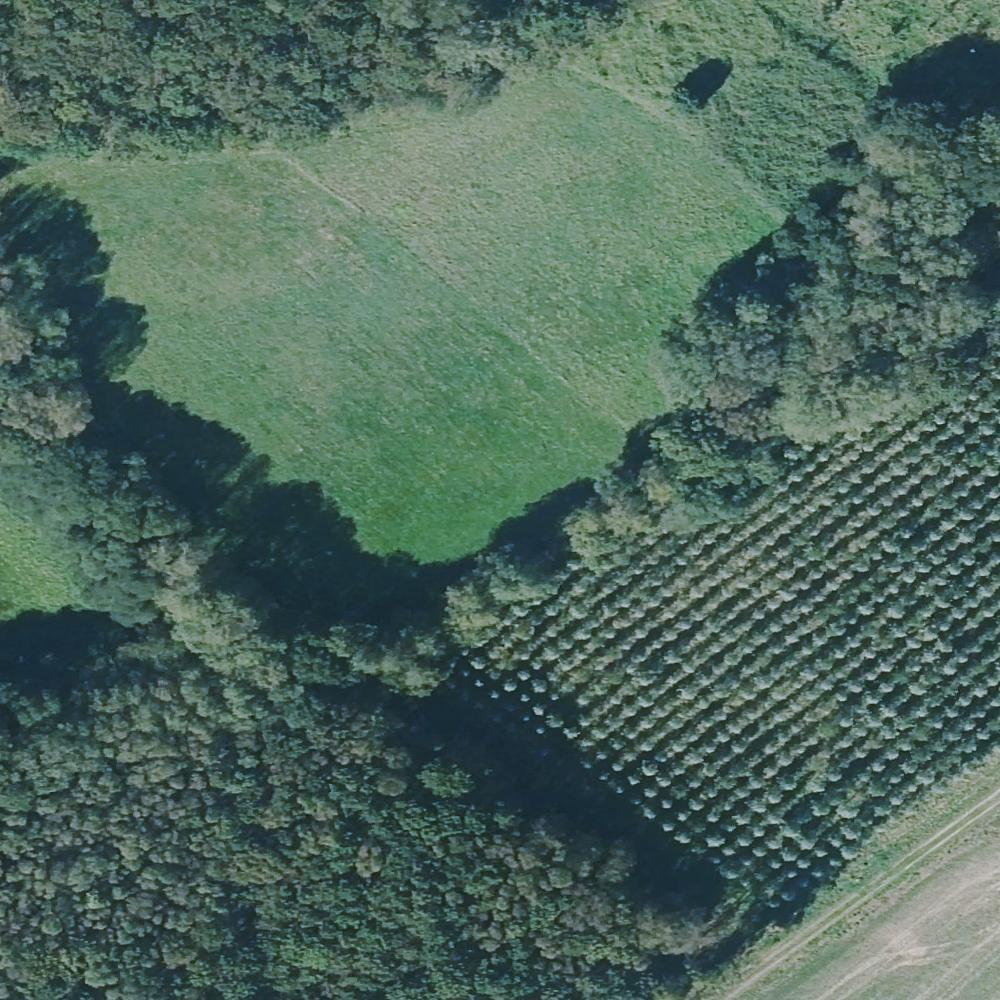
\includegraphics[width=\linewidth]{figuras/15_1903_1997.0.jpg}
        \label{fig:orto1}
    \end{subfigure}
    \hfill
    \begin{subfigure}[b]{0.31\textwidth}
        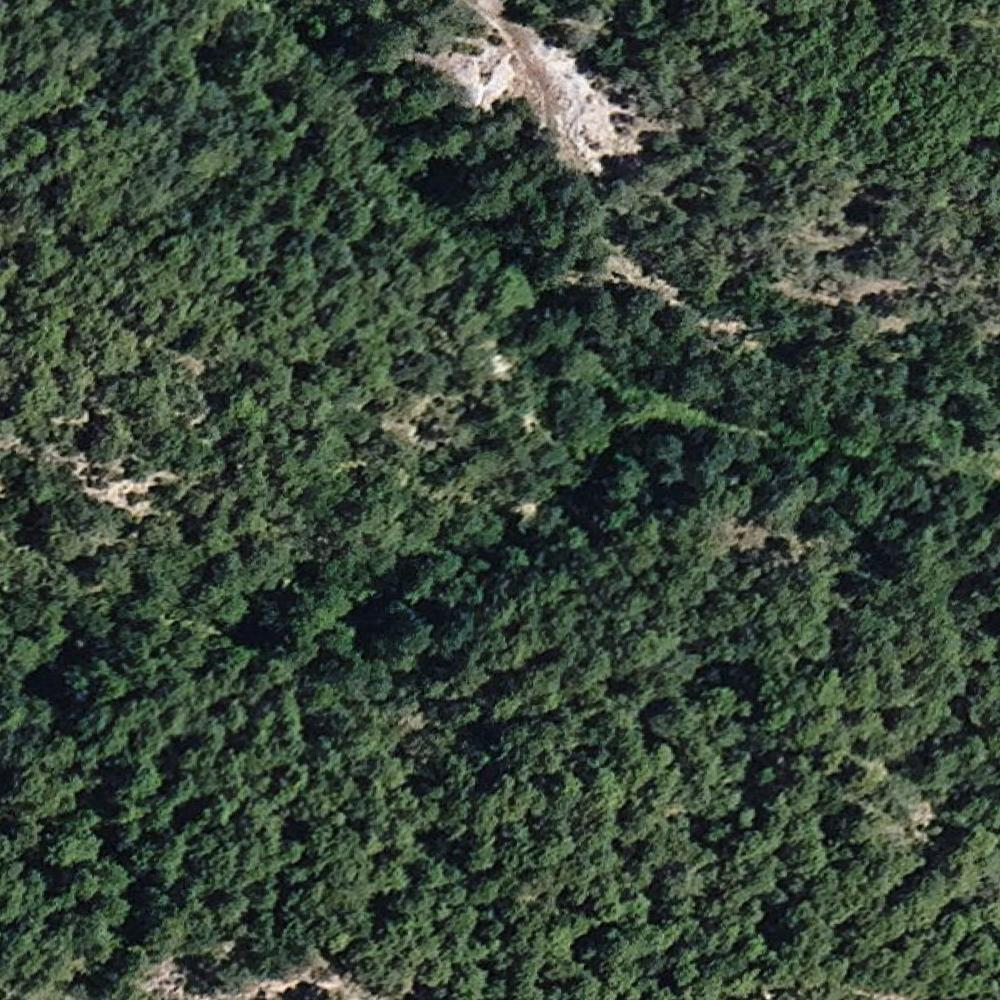
\includegraphics[width=\linewidth]{figuras/25_2209_2001.0.jpg}
        \label{fig:orto2}
    \end{subfigure}
    \hfill
    \begin{subfigure}[b]{0.31\textwidth}
        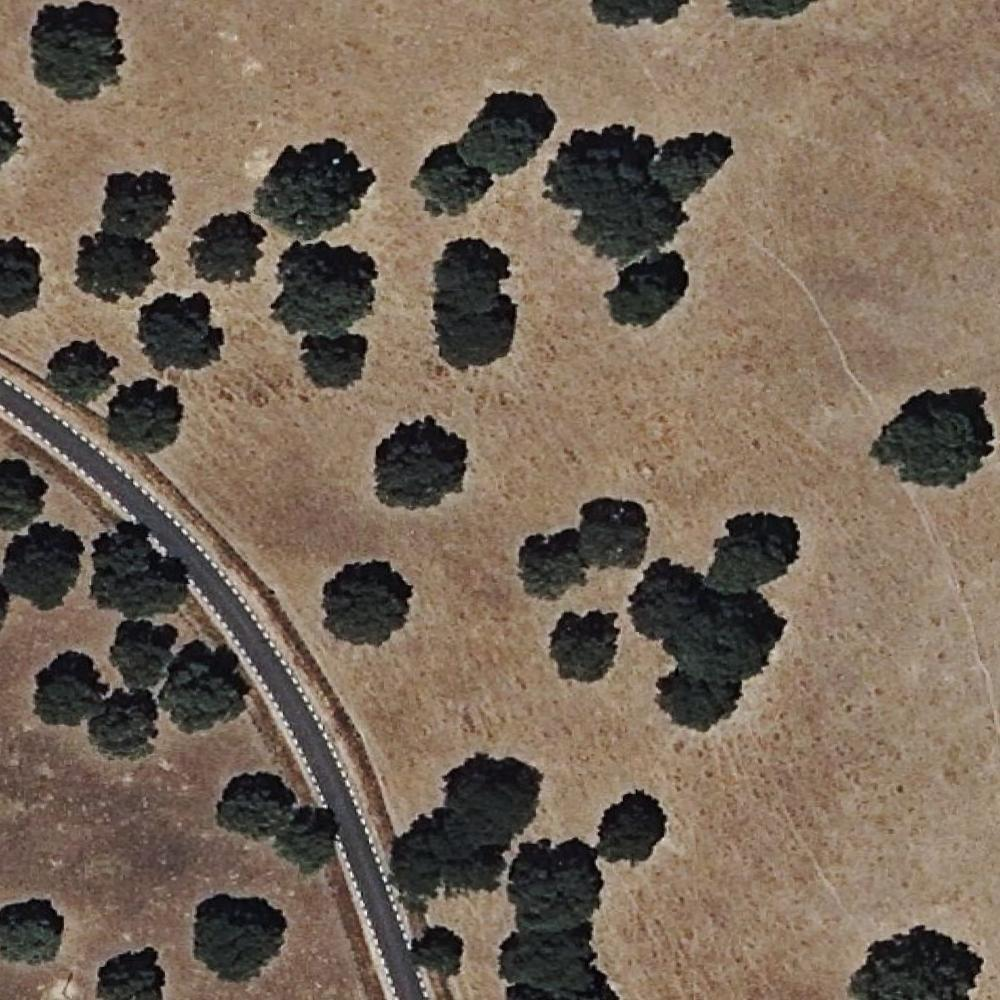
\includegraphics[width=\linewidth]{figuras/37_688_2002.0.jpg}
        \label{fig:orto3}
    \end{subfigure}
    
    \caption{\small Ejemplos de ortofotos del PNOA para tres parcelas del IFN. Se observa la cobertura arbórea y estructura del terreno con resolución submétrica. Estas imágenes fueron descargadas mediante peticiones WMS automatizadas en torno al centro geográfico de cada parcela.}
    \label{fig:ortofotos_ejemplo}
\end{figure}

